\documentclass{article}
\usepackage[utf8]{inputenc}
\usepackage[spanish,es-tabla]{babel}
\usepackage{graphicx}
\usepackage{float}


\title{Examen 1}
\author{Emilio Flores }
\date{Septiembre 2019}

\begin{document}

\maketitle
\begin{abstract}
    Este es un examen que pretende evaluar los conocimientos y uso del procesador de texto Latex, en este documento se pretende insertar una figura, una ecuacion, una tabla, un listado y referencias, donde todo debe ir con sus citas correspondientes dentro del texto.
\end{abstract}

\section*{Ecuación en Latex}
\begin{equation}
    v=v_0 - gt
    \label{eq1}
\end{equation}
\begin{equation}
    ma=-g
    \label{eq2}
\end{equation}
\begin{equation}
    x=x_0 + v_0t - gt^2
    \label{eq3}
\end{equation}

Las anteriores (\ref{eq1}, \ref{eq2}, \ref{eq3}) son son ejemplos de ecuaciones utilizadas en física.

\section*{Figuras en Latex}
\begin{figure}[H]
    \centering
    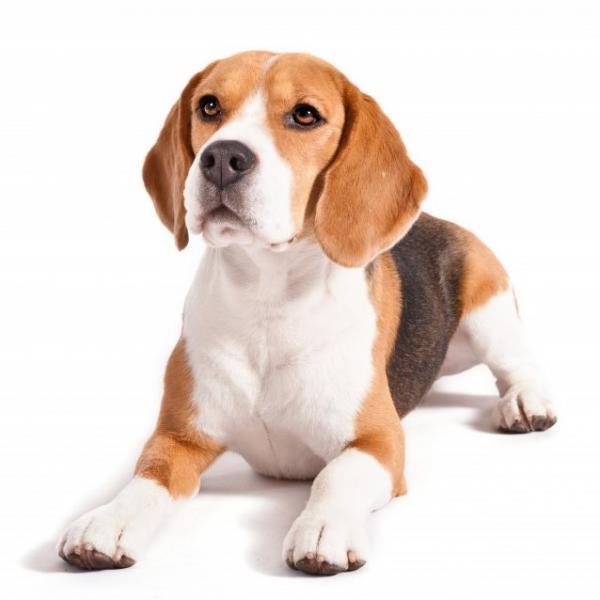
\includegraphics[scale=0.3]{fig1.png}
    \caption{Morris\label{fig1}}
    \end{figure}
    
    \begin{figure}[H]
        \centering
       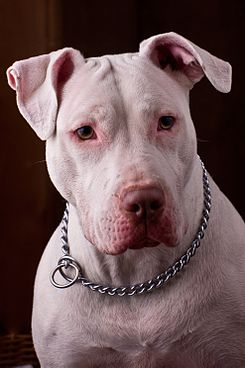
\includegraphics[scale=0.3]{fig2.png}
    \caption{Muñeca\label{fig2}}
\end{figure}

Las anteriores (\ref{fig1},\ref{fig2}) son figuras de mis perros en Latex.

\section*{Tablas en Latex}
\begin{table}[H]
    \centering
    \begin{tabular}{c|c|c}
    \hline\hline
       Posición  &  Velocidad & Tiempo\\ \hline\hline
        0.1 & 0.01 & 0.05\\
        0.2 & 0.04 & 0.10\\
        0.3 & 0.09 & 0.15\\
        \hline
    \end{tabular}
    \caption{Variación de la velocidad y el tiempo en función de la posición.}
    \label{t1}
\end{table}

Esta es una tabla en Latex (\ref{t1}).

\section*{Listados en Latex}

\begin{itemize}
    \item[a)] Primer paso
    \item[b)] Segundo paso
    \item[c)] Tercer paso
\end{itemize}

\begin{thebibliography}{2}
\bibitem{1} I. Newton, Principios matemáticos de la filosofía natural, (Ediciones Altaya,     Barcelona, 1993).
\bibitem{2} D.Halliday, R. Resnick y K.S. Krane. Física vol.1, (Compañía Editorial Continental. México DF, 1994).
\end{thebibliography}

Estos libros (\cite{1}, \cite{2}) comprenden mis referencias en el texto
\end{document}
